\chapter{Kvalitetssikring}\label{ch:Kvalitetssikring}

I dette afsnit gennemgås det, hvordan gruppen har kvalitetssikret projektet. Der er taget udgangspunkt i parametre fra FURPS+\cite{furps} og praktikker fra XP. Disse praktikker skal fungere i harmoni med Scrum, så kvaliteten af applikationen ikke tilsidesættes. Kvaliteten kan beskrives som værende primært ikke-funktionelle krav.

\section{FURPS+}
Som nævnt tidligere fokuserer agile udviklingsmetoder knap så meget på dokumentation, men mere på selve udviklingen af softwaren. Alt dokumentation, som ikke har en direkte indflydelse på softwaren, bliver nedprioriteret. Kvalitet i softwareudvikling omhandler koden mere end det gør andet. Kvalitetssikring kan beskrives ud fra FURPS+. FURPS står for Functionality, Usability, Reliability, Performance og Supportability. Hvor Functionality omhandler de funktionelle krav, så beskriver URPS de ikke-funktionelle krav. 
Usability omhandler bruger-oplevelsen (User Experience) - hvordan brugeren skal interagere med systemet for en optimal oplevelse og forståelse. Til dette kan brugergrænsefladen designes så den er intuitiv og responsiv, samt nem at navigere. 
Reliability omhandler sikkerhed til at systemet skal kunne håndtere fejl og uhensigtsmæssig brugeradfærd.
Performance omhandler responstid, tidsmål, og effektivitet af programmet. Dette ses som regel implementeret i form af Threads, Async/Await og refaktorering af kode.
Supportability omhandler vedligehold, videreudvikling og konfigurering. Dette ses ofte i form af dokumentation af funktionaliteten af programmet, decoupling af klasser og interfaces.

I dette projekt er der lavet refaktorering, som er omskrivning af kode med henblik på at optimere koden eller forståelsen af koden. Dette gør det nemmere at vedligeholde som nævnt under FURPS. 
Der er investeret tid i User Experience i dette projekt, sådan at front-end ikke bare er udelukkende funktionel, men også har overskueligt layout. Reliability er håndteret sammen med TDD fra XP, hvor der er taget højde for fejl-håndtering og sikkerhed. Der er lavet tests for de centrale services i projektet, herunder QWest.Api, og QWest.DataAccess, samt Model og Config. Disse tests er beskrevet mere nøje i programmerings- og teknologirapporten. Her er der sørget for at API og DAO har fungeret før det er blevet implementeret i systemet. Udover dette er der også taget højde for sikkerhed, i form af password hashing/salting, login-session, og den lagdelte struktur af programmet.
Programmet benytter sig af mange metoder, som kører asynkront, hvilket giver bedre performance end single-thread og med refaktorering bliver koden også optimeret efterhånden. Arkitekturen af programmet giver også god Supportability, da de forskellige services netop er services uafhængige af hinanden, og giver derfor god mulighed for implementering af nye features.

\section{XP praktikker}
Udover principperne fra FURPS, har praktikkerne fra XP også være en central del af projektet. Gruppen har tidligere besluttet at benytte procedurer fra XP til udviklingen af dette projekt, så procedurer som Pair Programming, Simple Design, Refactoring og Planning Game har gruppen sørget for at kvalitetssikre produktet. Til dette har Pair Programming og Test Driven Development\cite{Sommerville} haft en stor indflydelse på kvaliteten af produktet, da det øger Reliability og Supportability.
Under er der eksempler af hvordan teamet har benyttet procedurer fra XP til at kvalitetssikre produktet. 

\begin{figure}
    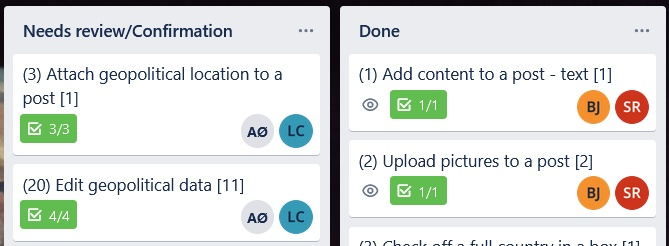
\includegraphics[width=\linewidth]{figures/pairprogramming.jpg}
    \caption{Eksempel af hvordan gruppen har benyttet Pair Programming fra XP.}
    \label{fig:Pair}
\end{figure}
Som det kan ses er der to gruppemedlemmer ansvarlig for hver opgave. Dette har hjulpet med at alle i gruppen fik en god forståelse for hvordan systemet er sammensat.


\begin{figure}
    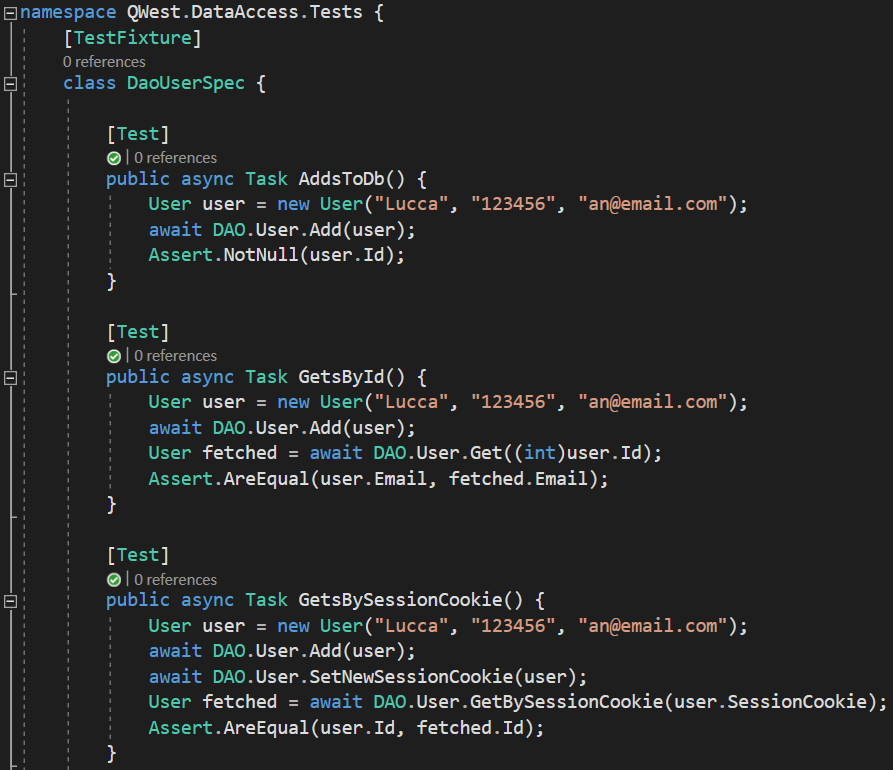
\includegraphics[width=\linewidth]{figures/tests2.png}
    \caption{Eksempel på test.}
    \label{fig:Test}
\end{figure}
Her ses et eksempel på opsætning af en test, med det klassiske Arrange, Act, Assert mønster. Dette mønster er blevet brugt under udviklingen af systemet, men tests bliver primært gennemgået i Programmerings- og Teknologirapporten.

\begin{figure}
    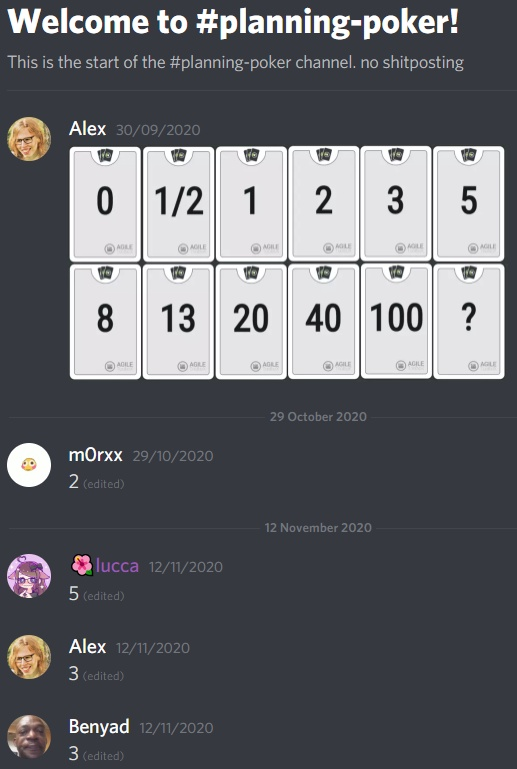
\includegraphics[width=\linewidth,scale=0.5]{figures/planningpoker.jpg}
    \caption{Eksempel på hvordan Planning Poker er benyttet gennem hele projektet.}
    \label{fig:Poker}
\end{figure}
Her ses det hvordan der i gruppen er lavet planningpoker. Hvert gruppemedlem har estimeret et antal timer, som bliver vist samtidigt efter en nedtælling. Hvis der er uenighed i estimaterne tages der en kort diskussion om hvad det bedste estimat ville være. Det er en nem, hurtig og sjov måde at planlægge sit sprint, og har fungeret godt i gruppen.
